\documentclass{article}
\usepackage[utf8] {inputenc}
\usepackage{hyperref}
\usepackage{graphicx}
\renewcommand{\baselinestretch}{1.2}
\title{Projektplanering CompoSink}
\author{Jonas Cronholm}
\date{September 2021}
\fontfamily{pcr}
\begin{document}
	\pagenumbering{Roman}
	\maketitle
	\pagebreak
	\tableofcontents
	\pagebreak

	\section{Projektbeskrivning}
	\subsection{Bakgrund och Mål}
	%	Vad har vi för mål? Hur kan vi konkretisera målet? [göra flera varianter för att man ska kunna installera produkten i kök, alla kök ör olika.]
	Vårt mål med projektet CompoSink är att utveckla en produkt som underlättar vardagen för de som har sin komposthink placerad på ett oåtkomligt eller på ett obekvämt ställe. Vår produkt ska underlätta detta genom att förflytta kompostnedkastet till en mer lättåtkomlig plats, nämligen precis bredvid eller nära diskhon. Vårt försäljningsmål för projektet är att utveckla och tillverka \textit{2500 enheter} i fyra olika varianter. Målet med de olika varianterna är att öka kompatibiliteten med olika placeringar i köket och olika storlekar för maximal kompatibilitet med alla kök. Vi anser att det är viktigt att tillverka an stor mängd av vår produkt så att vi kan lansera den i en stor skala. Till exempel att skicka ut visningsexemplar till vitvarubutiker såsom Elgiganten och Elon.
	\subsection{Budgetplanering}
	Vi uppskattar att projektet kommer att kosta ungefär:	
	\begin{figure}[h]
		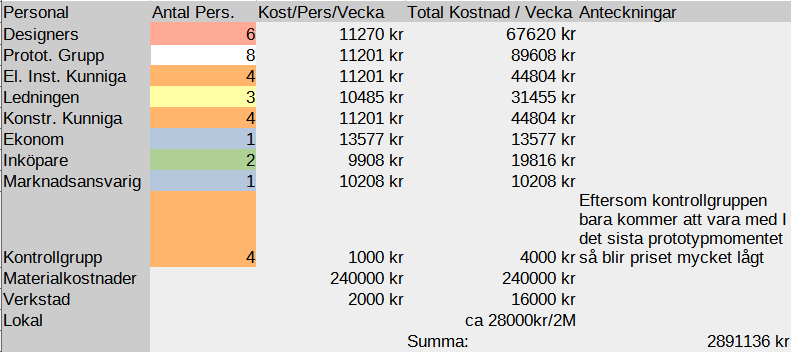
\includegraphics[width=\linewidth]{budget.png}
		\caption{Budget}
		\label{fig: BUDGET}
		\centering
	\end{figure}
	\subsection{Genomförande}
	Projektet är tänkt att genomföras genom att bygga ett team av kompetenta ingenjörer, designers, materialkunniga m.fl. och gemensamt utveckla en prototyp. Så att vi senare kan utveckla en marknadsredo produkt.
	\subsubsection{Efterforskning}
	För att vi ska kunna utveckla en produkt som framtidssäkras från konkurrens så måste vi ha en efterforskningsgrupp som efterforskar om tidigare försök för att framställa en liknande produkt har gjorts. Då kan vi lära oss av de misstagen som de ev. tidigare projekten gjorde under deras utvecklingsprocess.
	\subsubsection{Design}
	% För att vi ska kunna utveckla en produkt som tilltalar kunden så måste vi ha ett designteam som framställer flera olika produktvarianter som sedan kan presenteras till ledningen där beslut kan tas om den slutgiltiga versionen. 
	Våra designlag (se 1.5.1), kommer att framställa flera olika varianter som sedan presenteras för ledningen (Projektledaren m.fl.). Ledningen kommer att fatta ett beslut om vilken eller ev. vilka produktdesigns som kommer att vara den slutgiltiga design som vidarebefordras till prototyplaget (se 1.5.2). 
	\subsubsection{Prototyp 1, Extern design}
	Den första prototypen som kommer att tillverkas är den som kommer att användas för att projektledningen och eventuella kontrollgrupper (se 1.5.6) ska kunna få en klar bild på hur produkten kommer att se ut innan och efter den är monterad. Denna prototypen kommer att tillverkas "in-shop", detta innebär att projektets prototyputvecklingslag kommer att behöva ha tillgång till en verkstad där de kan arbeta med maskiner som t.ex. laserskärning, CNC-fräsning och eventuellt även injektionsgjutning. 
	\subsubsection{Elektronisk design}
	Den elektroniska designen kommer att skötas av det lag som byggts av de elektronikinstallationskunniga och deras främsta uppgift kommer att vara att utveckla den interna elektroniken som ser till att de olika elektroniska delarna fungerar som de ska enligt den ursprungliga idén. De elektronikinstallationskunniga kommer även att utveckla mjukvaran som kommer att köras på hårdvaran de utvecklar.
	\subsubsection{Prototyp 2, Intern design}
	Detta momentet är huvudsakligen till för att den interna designen av produkten ska vara lättarbetad av kunden (t.ex. att kunden ska kunna byta kompostpåsar snabbt och smärtfritt, eller att kunden ska kunna byta ut ev. förslitningsdelar som t.ex. kvarnknivbladen som maler ned komposten.). Under detta momentet kommer både design och propotyputvecklingslagen samarbeta för att utveckla de interna delarna av produkten. Även de elektronikinstallationskunniga kommer att behöva vara involverade eftersom det är i detta momentet som deras elektroniska delar kommer att monteras in i produkten. Detta innebär att den elektroniska designen måste vara klar innan prototypen börjar tillverkas.
	\subsubsection{Tester, felsökning, ev. ytterligare prototyp,}
	Testerna kommer att utföras för att säkerställa en användarvänlig och säker produkt. Felsökningen kommer vara på både hårdvarusidan och mjukvarusidan eftersom vi måste kunna garantera att produkten är felfri vid installation. 
	\subsubsection{Fabrikstillverkning}
	Fabrikstillverkningen kommer att ske när vi har en mycket väl fungerande prototyp som har presenterats för och godkänts av projektledningen. De konstruktionskunniga kommer då att bestämma ifall de kan producera \textit{2500} enheter med de resurser som de har fått tilldelade sig av ledningen, eller om de kommer att behöva skicka projektplanerna till en fabrik som har resurserna att producera enheterna.
	\subsubsection{Utdelning av informationsblad, manualdesign och Försäljning}
	För att vi ska kunna sälja \textit{2500} enheter till kunder och försäljare så måste vi dela ut information om produkten till div. partners. För att underlätta installation och underhåll av produkten så ska även en manual för produkten utvecklas.
	Informationsbladen som kommer att delas ut kommer innehålla all den information som försäljarna kommer att behöva för att kunna svara på kundernas frågor om produkten. 
	\subsubsection{Enkät}
	Enkäten som kommer att delas ut till kunderna har syftet att utvärdera kundernas upplevelser med produkten och att ge kunden en möjlighet att ge feedback till oss.
	\subsection{Uppföljning och Utvärdering}
	Vi kommer att mäta vårt resultat i antal enheter som vi har sålt till kunder och försäljare. \newline Utvärderingsprocessen kommer att bestå av en enkät som vi delar ut till våra kunder där de kan ge feedback på våran produkt och ge förslag till eventuella förbättringar.

	\subsection{Organisation}
	\subsubsection{Styrgrupp}
	Styrgruppen är den grupp som kommer att godkänna projektstart, olika projektfasers resultat och de kommer vara de som har sista ordet om en produktfunktion kommer att implementeras eller inte Styrgruppen följer det löpande arbetet och deltar i de eventuella beslut som skall tas under projektets gång.
	
	\subsubsection{Ansvar}
	Kunden tar ansvar för installation av produkten och eventuell felsökning om sådan skulle krävas. Dock kommer vi behöva ta ansvar för eventuella designproblem och tillverkningsfel.

	\subsection{Personer / Kompetenser / div. Resurser}
	%	Anställa folk med materialkompetens och designkunskaper för att utveckla produkten till en hållbar produkt som är lätt att installera.
	För att kunna utveckla våran produkt och producera den så kommer vi vara tvungna att anställa arbetskraft med specialkunskaper. Vi behöver produktdesigners, materialkunniga, elektronikinstallationskunniga och folk med egen erfarenhet från det problemet som vi försöker lösa, att ta hjälp av personer som har samma problem är bra eftersom alla kan ha olika infallsvinklar på problemet som gör att vi hittar fler smarta lösningar och så att vi kan arbeta snabbare.
	\begin{description}
		\item[Designlag] Designlagen kommer att ha ansvaret över att designa produkten. De kommer att arbeta i flera olika grupper som gemensamt framställer minst tre olika designalternativ av produkten som kan läggas fram till ledningen. \textit{Minst sex olika designers kommer alltså att anställas, högkompetenta designers krävs inte.}
		\item[Elektronikinstallationskunniga] De elektronikinstallationskunniga kommer att ha ansvaret över den elektroniska delen bakom CompoSink, även mjukvaran som kommer att köras på mikroprocessorerna kommer att utvecklas av denna gruppen. \textit{Personal med erfarenhet inom både hårdvara och mjukvara kommer alltså behövas anställas.}\pagebreak
		\item[Ledningen] Ledningen kommer att ha ansvaret över projektet. De kommer att se till att de olika lagen och teamen utför sina tilldelade uppgifter i tid. Ledningen kommer även att se över de olika prototyperna som kommer tillverkas och se till att dessa håller en viss kvalitet \textit{Ledningen kommer att behöva ha tidigare erfarenhet inom projektplanering, ledning och agil projektledning. Ledningen kommer inte behöva bestå av mer än fem personer.}
		\item[Konstruktionskunniga] De konstruktionskunniga kommer inte att delta i projektet förrän vi har en fungerande slutprototyp. \textit{De kommer att vara ansvariga för hela produktionscykeln och ev. för kommunikation med fabriker.}
		\item[Ekonom] För att vi ska kunna planera projektets ekonomi kommer vi att behöva anställa en ekonom som kan uppskatta momentens kostnad och anställningskostnaderna för de involverade i projektet.
		\item[Inköpare] Inköparen kommer att arbeta med prototyputvecklingslagen och köpa in det material och de verktygen som grupperna kommer att behöva. Inköparen kommer att ha ansvar över att köpa in varor med den summa pengar de har blivit tilldelade. \textit{Inköparen kommer att behöva ha kunskap om ekonomisk planering}
		\item[Marknadsansvarig] Den marknadsansvarige kommer att ha ansvar över produktens försäljning
		\item[Kontrollgrupp] Kontrollgruppen är en grupp externa personer som då och då får tillfället att komma med förslag till produktutvecklingar om de ser några. \textit{Dessa kommer att behöva ha erfarenhet av problemet. De behöver dock inte ha några andra kompetenser.}
	\end{description}

	
	\pagebreak 
	\section{Tidsplan}
	Den tidsplan som vi uppskattar för detta projekt är som följande. Vi uppskattar att:
	\begin{description}
	\item[Efterforskning] ca 20 [timmar]
	\item[Design] ca 50-70
	\item[Prototyp 1, tillverkning] ca 40 
	\item[Prototyp 1, tester och felsökning] ca 20-30
	\item[Elektronisk Design] ca 60-100
	\item[Prototyp 2, tillverkning] ca 60
 	\item[Prototyp 2, tester och felsökning] ca 20-30
	\item[Ev. Ytterligare prototyp] ca 80
	\item[Manualdesign] ca 20 
	\end{description}
	Se GANTT-schemat nedan.
	\begin{figure}[h]
		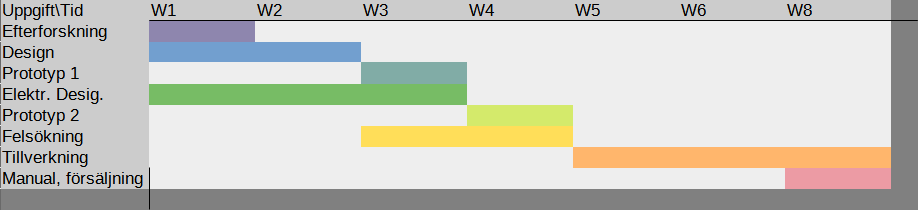
\includegraphics[width=\linewidth]{gantt1.png}
		\caption{GANTT-Schema, där W indikerar vecka}
		\label{fig: GANTT1}
		\centering
	\end{figure}
	
\end{document}